\documentclass[conference,compsoc,final,a4paper]{IEEEtran}
\usepackage[utf8]{inputenx}
\usepackage{float} % for Table float parameter H

%% Bitte legen Sie hier den Titel und den Autor der Arbeit fest
\newcommand{\autoren}[0]{Karhan, Marvin}
\newcommand{\dokumententitel}[0]{Welchen Einfluss haben Dark Patterns auf Nutzer?}

% Hie muss normalerweise nichts angepasst werden
\usepackage[pdftex]{graphicx}
\graphicspath{{img/}}
\DeclareGraphicsExtensions{.pdf,.jpeg,.jpg,.png}
\usepackage[cmex10]{amsmath}
\usepackage{algorithmic}
\usepackage{array}
\usepackage{dblfloatfix}
\usepackage{url}
\usepackage[autostyle=true,german=quotes]{csquotes}
\usepackage[backend=biber,
            sorting=none,   % Keine Sortierung
            doi=true,       % DOI anzeigen
            isbn=false,     % ISBN nicht anzeigen
            url=true,       % URLs anzeigen
            maxnames=6,     % Ab 6 Autoren et al. verwenden
            minnames=1,     % und nur den ersten Autor angeben
            style=ieee,]{biblatex}
\usepackage{booktabs}
\usepackage{xcolor}
\usepackage{listings}             % Source Code listings
\usepackage[printonlyused]{acronym}
\usepackage{fancyvrb}
\usepackage{tocloft} % Schönere Inhaltsverzeichnisse

% Farben definieren
\definecolor{linkblue}{RGB}{0, 0, 100}
\definecolor{linkblack}{RGB}{0, 0, 0}
\definecolor{darkgreen}{RGB}{14, 144, 102}
\definecolor{darkblue}{RGB}{0,0,168}
\definecolor{darkred}{RGB}{128,0,0}
\definecolor{comment}{RGB}{63, 127, 95}
\definecolor{javadoccomment}{RGB}{63, 95, 191}
\definecolor{keyword}{RGB}{108, 0, 67}
\definecolor{type}{RGB}{0, 0, 0}
\definecolor{method}{RGB}{0, 0, 0}
\definecolor{variable}{RGB}{0, 0, 0}
\definecolor{literal}{RGB}{31,0, 255}
\definecolor{operator}{RGB}{0, 0, 0}

\usepackage[ngerman]{betababel}

\DefineBibliographyStrings{ngerman}{
    andothers = {{et al\adddot}},  % Immer et al. sagen, auch bei Deutsch als Sprache
}
\usepackage[
      unicode=true,
      hypertexnames=false,
      colorlinks=true,
      colorlinks=false,
      linkcolor=darkblue,
      citecolor=darkblue,
      urlcolor=darkblue,
      pdftex
   ]{hyperref}
%	 \PrerenderUnicode{ü}


% Einstellungen für Quelltexte
\lstset{
    xleftmargin=0.1cm,
    basicstyle=\scriptsize\ttfamily,
    keywordstyle=\color{keyword},
    identifierstyle=\color{variable},
    commentstyle=\color{comment},
    stringstyle=\color{literal},
    tabsize=2,
    lineskip={2pt},
    columns=flexible,
    inputencoding=utf8,
    captionpos=b,
    breakautoindent=true,
    breakindent=2em,
    breaklines=true,
    prebreak=,
    postbreak=,
    numbers=none,
    numberstyle=\tiny,
    showspaces=false,      % Keine Leerzeichensymbole
    showtabs=false,        % Keine Tabsymbole
    showstringspaces=false,% Leerzeichen in Strings
    morecomment=[s][\color{javadoccomment}]{/**}{*/},
    literate={Ö}{{\"O}}1 {Ä}{{\"A}}1 {Ü}{{\"U}}1 {ß}{{\ss}}2 {ü}{{\"u}}1 {ä}{{\"a}}1 {ö}{{\"o}}1
}

\hypersetup{
    pdftitle={\dokumententitel},
    pdfauthor={\autoren},
    pdfdisplaydoctitle=true,
    hidelinks
}

% Makros für typographisch korrekte Abkürzungen
\newcommand{\zb}[0]{z.\,B.\ }
\newcommand{\dahe}[0]{d.\,h.\ }
\newcommand{\ua}[0]{u.\,a.\ }

% Wo liegt Sourcecode?
\newcommand{\srcloc}{src/}

% Literatur einbinden
\addbibresource{literatur.bib} % Weitere Einstellungen aus einer anderen Datei lesen

\begin{document}

% Titel des Dokuments
\title{\dokumententitel}

% Namen der Autoren
\author{
  \IEEEauthorblockN{\autoren}
  \IEEEauthorblockA{
    Hochschule Mannheim\\
    Fakultät für Informatik\\
    Paul-Wittsack-Str. 10,
    68163 Mannheim
  }
}

% Titel erzeugen
\maketitle
\thispagestyle{plain}
\pagestyle{plain}

% Eigentliches Dokument beginnt hier
% ----------------------------------------------------------------------------------------------------------

% Kurze Zusammenfassung des Dokuments
\begin{abstract}
Abstract
\end{abstract}

% Inhaltsverzeichnis erzeugen
{\small\tableofcontents}

% Abschnitte mit \section, Unterabschnitte mit \subsection und
% Unterunterabschnitte mit \subsubsection
\section{Einleitung}
"“Dark pattern” means a user interface designed or manipulated with the substantial effect of subverting or impairing user autonomy, decisionmaking, or choice"

Mit der immer stärker zunehmender Digitalisierung und der steigenden Anzahl an Internet Nutzern \autocite{ITU2020}, wird der Einfluss von Applikationen im Internet und ihrem Design immer größer. Für ihre Nutzer ist es nicht immer klar, wenn sie ausgenutzt worden. Menschen sind besonders gut in der Erkennung von Mustern, wir nutzen die muster verschiedener Laute Sprache verstehen und sprechen zu können. Deshalb ist es wichtig zu verstehen welche Muster im Internet eingesetzt werden, um uns zu beeinflussen.

Viele Gelehrt befassen sich damit Richtlinien und Vorlagen für gutes Interface Design zu verfassen. Dieses Paper beleuchtet die dunkle Seite des Interface Designs im Webumfeld. Von besonderer Bedeutung ist dabei der Einfluss von \textit{Dark Patterns} auf Nutzer. Sie sind Negativbeispiele für Interface Design und dienen nicht dem wohle der Nutzer. Harry Brignull gilt als der Begründer des Dark Pattern Begriffs und definiert ihn als Tricks die Nutzer dazu überzeugen etwas zu tun, was sie ursprünglich nicht tun wollten \autocite{Brignull}. Sie nutzen Psychologische Mechanismen, um die Entscheidungsfindung des Nutzers wesentlich zu beeinflussen.

Das Ziel dabei ist zweiseitig, einerseits soll es Designern leichter fallen Dark Patterns in ihren Designendscheidungen zu vermeiden und anderseits sollen Nutzer leichter in der Lage sein Dark Patterns zu erkennen, um so negative Konsequenzen zu verhindern. 

% Umfang und Abgrenzung 
Diese Arbeit bietet einen Einblick in die Konzepte, die das Fundament für Dark Patterns bilden und welche rolle dabei psychologische Mechanismen einnehmen. Außerdem werden Beispiele von Dark Patterns in die von \citeauthor{Gray_2018} etablierte Taxonomie eingeordnet und bewertet. Zudem werden Legislative Maßnahmen gegen Dark Patterns betrachtet und beantwortet die Frage, wieso die Aufklärung von Designern und Nutzern nötig ist.
% Dieses Paper vermittelt einen Einblick in die Konzepte, die das Fundament für die Definition des Dark Pattern Begriffes liefern. Wie sich Dark Patterns in Applikationen manifestieren und wie Verbraucher vor Missbrauch durch Dark Patterns geschützt werden, bzw. wie können sich Nutzer davor schützen. Außerdem wird im Ausblick darauf eingegangen wie Regularien oder Nutzerverhalten den Einsatz von Dark Patterns in Zukunft beeinflussen kann.

% Format und Struktur (irgendwie schon im vorherigen absatz geklärt..?)

% \section{Zusätzliche Angaben}
% \subsection{Zentrale Begriffe}
% \begin{itemize}
% \item Dark Pattern
% \item Anti-Pattern
% \item evil design
% \item black hat UX
% \item dark ux
% \item Marktpsychologie
% \item CCPA (California Consumer Privacy Act)
% \item GDPR (General Data Protection Regulation)
% \item Persuasive design
% \item Deceptive design
% \item Human-centered computing
% \item Human computer interaction (HCI)
% \end{itemize}

% \subsection{Zeitplan}
% Generell ist vor jeder textuellen Abgabe entsprechend dem Umfang der Abgabe eine Rechtschreibprüfung eines Dritten angesetzt.
% \begin{table}[H]
% \begin{tabular*}{\linewidth}{ @{\extracolsep{\fill}}l  l}
%     \toprule
% \textbf{Zeitraum}                   & \textbf{Geplante Tätigkeit}       \\
%     \midrule
% 16.04 - 23.04                       & Weitere Literaturrecherche        \\
% 24.04 - 30.04                       & Kapitel 3.0 (Kapiteleinleitung), 3.1                          \\
% 01.05 - 14.05                       & Kapitel 3.2 - 3.4                          \\
% \textbf{14.05}                      & \textbf{Abgabe des Probekapitels} \\
% 15.05 - 28.05                       & Kapitel 4                           \\
% 29.05 - 11.06                       & Kapitel 5                          \\
% 12.06 - 25.06                       & Kapitel Abstract und Einleitung                          \\
% \textbf{25.06}                      & \textbf{Abgabe zum Peer-Review}   \\
% \textbf{07.07}                      & \textbf{Peer-Review (8:00 - 11:15 Uhr)} \\
% \textbf{08.07}                      & \textbf{Abgabe der Peer-Review-Bögen}   \\
% 09.07 - 16.07                       & Einarbeitung der Kritik und letzte Verbesserungen                           \\
% \textbf{16.07}                      & \textbf{Abgabe des fertigen Papers}      \\
%     \bottomrule
% \end{tabular*}
% \end{table}

% \subsection{Kontextabgrenzung}
% Dieses Paper vermittelt einen Einblick in die Konzepte, die das Fundament für die Definition des Dark Pattern Begriffes liefern. Wie sich Dark Patterns in Applikationen manifestieren und wie Verbraucher vor Missbrauch durch Dark Patterns geschützt werden, bzw. wie können sich Nutzer davor schützen. Außerdem wird im Ausblick darauf eingegangen wie Regularien oder Nutzerverhalten den Einsatz von Dark Patterns in Zukunft beeinflussen kann.

\section{Dark Patterns Grundlagen}
% // David Brignull als Erfinder des Begriffs 2010\\
% // wer setzt das warum ein\\
//Neuer Einstieg\\

Traditionell nutzen Firmen Plakate und Anzeigen um Kunden auf sich aufmerksam zu machen. Durch die Entstehung des Internets verbreitete sich das sogenannte \textit{Growth Hacking}. Mit Growth Hacking werden Marketing Aktionen bezeichnet, welche Tricks ausnutzen, um Wachstum zu steigern. Growth Hacks bewegen sich häufig an der Grenze zum illegalem  \autocite{Narayanan2020}. LinkedIn gab seinen Nutzern die Möglichkeit automatisiert persönliche Kontakte per E-Mail zu LinkedIn einzuladen. Sie nutzten diese Einwilligung, um wiederholt E-Mails im Namen der Nutzer an deren Kontakte zu senden. Daraus resultiere eine Sammelklage, da es für die Nutzer nicht klar war das LinkedIn die Kontakte im Namen des Nutzers mit werbe Mails spammen würde \autocite{Strange2015}. Solche Marketing Aktionen sind der Urstprung von Dark Patterns. 

Dieses Kapitel ordnet Dark Patterns ein, beschreibt wie die menschliche Psyche ausgenutzt werden kann, was \textit{Nudging} ist und anhand eines Beispiels wie \textit{Nudges} eingesetzt werden können.
\subsection{Anti-Pattern}
% // Anti-Pattern als Überbegriff von Dark Pattern und Einleitung in das Thema\\
Pattern sind der Bauplan einer Lösung zu einem wiederkehrenden Problem. Sie existieren in vielen Anwendungsbereichen \autocite[S. 1]{MacDonald2019}.

Anti-Pattern sind ist Sammelbegriff für Pattern, welche wiederkehrende Lösungen liefern, aber dabei mehr Probleme erzeugen als lösen \autocite[S. 193-195]{MacDonald2019}. Wie sich aus dem Namen bereits erschließen lässt, sind Dark Patterns eine spezifische Pattern-Art.
Unternehmen setzen Dark Pattern ein um, ihre Reichweite zu erhöhen. Das Schafft Probleme aufseiten der Nutzer, da der Nutzer ausgenutzt und Profit über Nutzerfreundlichkeit gestellt wird \autocite{Chivukula_2019}, zählen Dark Patterns zu der Familie der Anti-Pattern.
\subsection{Psychologie}
\label{chap:Psychologie}
% // Warum spielt Psychologie eine rolle bei Dark Patterns?
% \\// Wie werden Nutzer von Dark Pattern beeinflusst?
% \\// Diskussion verschiedener erhobenen Statistiken zu Nutzerverhalten:\\
Dark Patterns nutzen Psychologische Mechanismen aus, um Nutzer zu bewegen, etwas ungewollt oder unbewusst zu tun \autocite{Brignull}. Dafür nutzen sie oft kognitive Verzerrung, nutzen also mit speziellen Techniken die Denkweise unseres Gehirns aus \autocite{Mathur2019}.

Eine weitverbreitete Technik im Einzelhandel ist die psychologische Preisgestaltung. Das heißt der Preis eines Produkts wird knapp, unter einer runden Zahl angesetzt. Diese Technik ist schon seit mehreren Jahrzehnten im Einsatz und laut \citeauthor{Bizer_2005} (\citedate{Bizer_2005}) \autocite{Bizer_2005} ein effektives Mittel zur Verkaufssteigerung. Im Gegensatz dazu steht \citeauthor{Wieseke_2015} \autocite{Wieseke_2015} Studie aus dem Jahr \citedate{Wieseke_2015}, die sagt: Runde Preise sorgen für die höchstmögliche Verkaufswahrscheinlichkeit, da diese bequemer für den Käufer sind. Ein vergleichbarer Effekt kann bei Dark Patterns auftreten. Im ersten Schritt sorgt der Einsatz von Dark Patterns für eine höhere Nutzerbindung, jedoch im zweiten Schritt zu einer gegenläufigen Wirkung \autocite{M.Bhoot2020}.

Schon in der Zeit vor der Digitalen Revolution wurden die Effekte kognitiver Verzerrung untersucht. Die Ergebnisse dieser Untersuchungen geben Aufschluss über die Manifestierung von Dark Patterns in der menschlichen Psyche.

\citeauthor{Tversky453} zeigen in ihrer Untersuchung \autocite{Tversky453}, wie die Darstellung eines Problems das Ergebnis beeinflusst: Probanden treffen eine andere Auswahl, obwohl sich nur die Darstellung des Problems geändert hat. Konkret mussten die Probanden im ersten Problem konsekutiv eine aus Zwei Möglichkeiten wählen, dabei handelte es sich, um die Chance Geld zu gewinnen oder zu verlieren. In einem anderen Problem wurden die zwei meist gewähltesten so wie die anderen zwei anderen Optionen zusammengefasst. Nach der Kombinierung der zwei Aussichten entschieden sich 100\% auf die vorher kaum gewählten Optionen. Diese psychologische Betrachtung lässt sich leicht auf Dark Patterns ausweiten, da Designer in einem Webumfeld weitreichende Möglichkeiten haben, um Information, so zu vermitteln, dass der Nutzer nur durch ihre Darstellung zu einer anderen Entscheidung gedrängt wird.
\subsection{Nudging}
% // Vorhersehbares Beeinflussen von Nutzern um ein gewünschtes Ziel zu erreichen\\
Richard H. Thaler ist Nobelpreisträger für Wirtschaftswissenschaften. Er ist zusammen mit Cass R. Sunstein der Autor des Buchs \citetitle{Thaler2008} \autocite{Thaler2008}, der den Begriff \textit{Nudge} geprägt hat.

Er bezeichnet Personen, die Macht über den Kontext haben, indem Andere Entscheidungen treffen als \textit{choice architects} \autocite[S. 3]{Thaler2008}. Im Fall von Dark Patterns sind meistens Designer diejenigen, die Thaler und Sunstein als \textit{choice architects} bezeichnen. Ihre Werkzeuge sind die psychologischen Effekte und Techniken.

\textit{To nudge} bedeutet im herkömmlichen Sinne, jemanden sachte berühren oder schubsen \autocite{MerriamWebsterNudge}. Wir werden den Begriff wie Thaler und Sunstein im übertragenen Sinne nutzen, wobei \textit{nudge} meint jemanden mithilfe kleiner Anreize zu einem wünschenswerten Ziel zu drängen. Denn schon mit nur kleinen Anreizen kann der Nutzer zu einer anderen Entscheidung gedrängt werden \autocite{Narayanan2020}.

\begin{figure}[!ht]
\centering
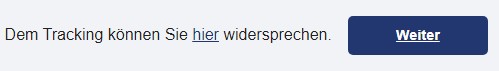
\includegraphics[width=\linewidth]{hochschule_cookie_banner}
\caption{Eigene Aufnahme des Tracking-Banners der Hochschule Mannheim~\autocite{HSMAWebsite2021}}
\label{fig:HSMATracking}
\end{figure}

\begin{figure}[!ht]
\centering
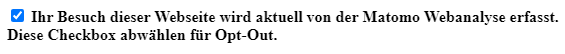
\includegraphics[width=\linewidth]{tracking_optout}
\caption{Eigene Aufnahme der Tracking Opt-Out Checkbox der Hochschule Mannheim~\autocite{HSMAWebsite2021}}
\label{fig:HSMAOptOut}
\end{figure}

Um \textit{Nudging} besser zu verstehen, betrachten wir ein Dark Pattern, welches sich auf der Homepage der Hochschule Mannheim finden lässt. In \autoref{fig:HSMATracking} ist ein Ausschnitt des Tracking-Banners der Hochschule Mannheim zu sehen. Die Zustimmung zu nicht essenziellem Tracking wird hinter einem prominent dargestelltem \textit{Weiter} Button verborgen. Um eine konträre Entscheidung zu treffen, muss der Nutzer auf den weit weniger prominenten \textit{hier} Link klicken. Dieser führt zu der Datenschutzerklärung der Hochschule in der nach der in \autoref{fig:HSMAOptOut} dargestellten Checkbox gesucht werden muss, um das Tracking zu deaktivieren. Auffällig ist, dass in dem Text das Wort \textit{tracking} nicht vorkommt. Hier wurden mehrere \textit{Nudges} genutzt, um den Nutzer dazu zu bewegen, das Tracking zu akzeptieren. Erst wird der Nutzer zum direkten Akzeptieren durch einen auffälligeren Button \textit{genudged}, danach wird der Nutzer durch das erschwerte Abwählen des Trackings in Richtung der Akzeptanz des Trackings \textit{genudged}.

Zusammenfassend lässt sich sagen, dass Dark Patterns als Zusammenschluss verschiedener Nudges verstanden werden kann.

\section{Kategorien von Dark Patterns}
//Bilder aus Kapitel 3. Nudging (HSMA) einordnen + zweites Dark Pattern (confirm shaming) direkt über
\autoref{fig:HSMAOptOut}\\
// Taxonomy mit verschiedenen Quellen belegen \autocite*{Gray_2018,M.Bhoot2020,Brignull}


\subsection{Nagging}
// Nerven bis man ja sagt (Z.B. iPhone Apple Pay-Einrichtung or No Button for No)
\subsection{Obstruction}
\label{chap:Obstruction}
// Verbergen von Information durch Design, z.B. wenn ein Shop immer direkt die teuerste Variante (farblich) eines Produkts zeigt
\\// Roach motel, easy to enter hard to leave
\subsection{Sneaking}
// Versteckte Kosten, sneak into basket, versteckte Subscriptions, z.B. hinter einem free trial
\subsection{Interface Interference}
// Manipulation of the user interface that privileges certain actions over others.
\subsection{Forced action}
// Wenn man gezwungen wird, etwas zu tun, was man nicht will und was nicht erforderlich ist, z.B. Annehmen eines Newsletters zur Anmeldung oder das Liken einer Seite, um sie zu besuchen


\section{Schutz vor Dark Patterns}
// hier fehlt noch etwas zum Gesetz und Designern.\\
Nutzer lesen nicht jedes Wort auf einer Webseite, sie überfliegen und machen Annahmen \autocite{Brignull}. Firmen können das ausnutzen, indem sie die Seite anders aussehen lassen, als was sie tatsächlich aussagt \autocite{Brignull}.

Designer müssen viele Entscheidungen bei dem Designen einer Webseite treffen. Im digitalen Umfeld wird dafür häufig A/B-Testing eingesetzt, da so Annahmen mit Nutzerdaten untermauert werden können. Das führt häufig dazu, dass Designer unbewusst und ohne eine böse Absicht Dark Patterns in die Webseite einbinden \autocite{Narayanan2020}.

\subsection{Gesetzliche Einschränkungen}
// Self-regulate or get regulated
\\// genauer Gesetzes Auszug aus dem (CCPA) \begin{quotation}Cal. Civ. Code § 1798.140(l)\end{quotation}
\subsection{Designer-Aufklärung}
// Entwickler entwickeln oft Dark Patterns ohne dass ihnen das bewusst ist
\subsection{Nutzer-Aufklärung}
// subreddit '/r/assholedesign' \autocite{Chivukula_2019}\\
// Brignull klärt auf seiner Seite auf \autocite{Brignull}
// Nutzer aufklären, führt zur Reduzierung des Erfolges von Dark Patterns, was wiederum dafür sorgt, dass Dark Patterns sich für Firmen weniger lohnen und sie auf diese verzichten\\
Laut \citeauthor{Brignull} \autocite{Brignull} ist der beste Schutz vor Dark Patterns, sie sich bewusst zu machen und die Firmen, die sie benutzen zu boykottieren. \autoref{chap:Psychologie} zeigt, dass der Mensch anfällig für Dark Patterns sein kann. 41.4\% der Befragten einer Studie von \citeauthor{M.Bhoot2020} \autocite{M.Bhoot2020} gaben an noch nie von einer Webseite ausgetrickst worden zu sein, jedoch hat keiner der Befragten alle zwölf Dark Pattern der Studie identifizieren können. \citeauthor{M.Bhoot2020} identifizieren Auftrittshäufigkeit als wichtigsten Gesichtspunkt zur Identifikation von Dark Pattern. Deshalb ist es wichtig, Nutzer über Dark Patterns aufzuklären, sodass sie diese leichter erkennen, um sich selbst vor ungewollten Konsequenzen schützen können.

Ein bedeutendstes Merkmal zur Erkennung von Dark Patterns ist die Auftrittshäufigkeit \autocite{M.Bhoot2020}. -> sub-Reddit


In der Fußgängerzone stellen Hütchenspieler ihrem Publikum hohe Gewinnchancen in Aussicht, naive Passanten verstehen es als Geschicklichkeit spiel dessen Ausgang sie durch ihr Können bestimmen, jedoch ist das ein Irrtum. Der Hütchenspieler nutzt einfache Taschenspielertricks und kontrolliert jederzeit den Ausgang des Spiels. 

\section{Fazit und Ausblick}

% Literaturverzeichnis
\addcontentsline{toc}{section}{Literatur}
\printbibliography
\end{document}
// bill zitieren mit namen